\subsection{Content Server} \label{section:counter-replace-server}
This approach is to fight the shortcomings of the license verification libraries by moving them to a server.
Users have to login on a server in order to verify their license.
Instead of returning just the result of the verification, the server delivers part or all of the content of the application.
Since license verification no longer is dependent on an unary result, \gls{luckypatcherg} fails.
The content provided by the server cannot be second guessed by \gls{luckypatcherg}.
\newline
\begin{figure}[h]
    \centering
    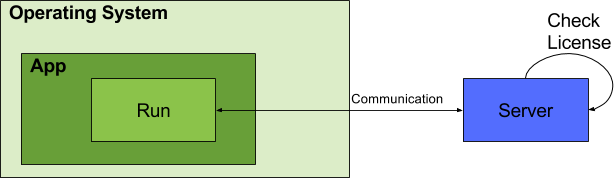
\includegraphics[width=0.8\textwidth]{data/contentServer.png}
    \caption{Abstraction of an application and a content server}
    \label{fig:contentServer}
\end{figure}
The implementation can be described with the application Spotify \cite{spotify} as an example.
Instead of verifying the license locally on the device, the user has to enter his credentials and send them to the server.
In case the credentials are valid, the user is logged into the application.
The content, the music in this case, is no longer on the phone itself, but streamed from the server.
The attacker still can circumvent the login process inside the application by manipulating the code.
Since the content is on the server and the user has to be authorized on it, no content is available inside the application.
Thus attacks on the applications itself do not work anymore.
\newline
\newline
In general, a content server is a solution against piracy, but it has downsides as well.
The first problem is that this architecture cannot be applied to all applications.
This means that it must be possible to extract parts of the application's logic and implement them on a server.
This is not possible for all applications.
\newline
The second problem are the additional resources needed.
When outsourcing parts of the application on a server, not only money is needed for the server, but an additional application for the server has to be created.
Not every developer can handle this additional workload.
\newline
The third problem is the always online necessity.
It limits the freedom of users and creates additional internet traffic.
This is not accepted by all users.
\newline
\newline
Nevertheless, if this implementation can be realized, it is safe from \gls{luckypatcherg} auto patching as well as custom patches.
In addition, when the core algorithm is moved to the server this mechanism protects the developers \gls{ip}.
This prevents attackers not only from using the application for free, but also from reconstructing the the core functionality and implementing it somewhere else.
